\chapter{Dual Radar Fusion Pipeline}
This chapter explores the core engineering of the project: the real-time software pipeline that synchronizes, calibrates, and fuses two independent radar point clouds into a single unified spatial frame.

\section{Frame Synchronization}
Because the two IWR6843AOP units operate on independent internal clocks with no hardware synchronization, their incoming frames must be aligned in software. 
When each frame arrives via USB, the host computer tags it with a wall-clock timestamp and places it into a ring buffer. A dedicated pairing thread continuously inspects the queues of both Radar A and Radar B. It matches frames that have the smallest time difference. If the absolute time difference $|\Delta t|$ is below 50 ms (half of the 100 ms frame period), the pair is accepted and forwarded to the calibration pipeline. Unmatched frames are discarded to prevent queue buildup and latency.

\section{Auto-Calibration: SVD + RANSAC}
Every sensor defines its origin $(0,0,0)$ relative to its physical placement. To convert points from Radar B into Radar A's coordinate system, we must dynamically compute a rigid transform consisting of a 3x3 rotation matrix ($R$) and a 3D translation vector ($t$).

\subsection{Collecting Correspondences}
A correspondence is formed when both radars track the same person simultaneously. To collect data, a person walks through the overlapping field of view for 20–30 seconds, generating paired target centroids $\{p_A, p_B\}$. 

\subsection{SVD Decomposition}
Once sufficient pairs (typically $>$15) are collected, both point sets are centered by subtracting their respective means ($\mu_A, \mu_B$). A cross-covariance matrix $H$ is computed from the centered points. Applying Singular Value Decomposition (SVD) to $H$ yields matrices $U, S$, and $V$. The optimal rotation matrix is obtained analytically via $R = V \times U^T$. The translation vector is then derived as $t = \mu_B - R \times \mu_A$. SVD guarantees a globally optimal rotation in microseconds without iterative guessing.

\subsection{RANSAC Inlier Filtering}
Because radar tracking can occasionally assign tracks to multipath ghosts, the raw correspondence set often contains outliers. Random Sample Consensus (RANSAC) is employed to isolate the true geometry. RANSAC repeatedly samples 4 random pairs, computes a candidate $(R, t)$, and tests all other pairs for reprojection error. The candidate transform that yields the highest consensus (inliers with $<0.2$ m error) is selected. A final SVD pass is performed exclusively on these inliers.

\subsection{Drift Detection and Auto-Recalibration}
During live operation, the system continuously compares the transformed Radar B target centroid against the Radar A target centroid. If the mean disagreement exceeds 0.3 m for ten consecutive frames, the system assumes a sensor was physically bumped or moved. It automatically pauses fusion, collects a fresh set of correspondence pairs, executes SVD+RANSAC, and resumes operation with the new $(R, t)$ matrix. This self-healing loop operates entirely without human intervention.

Figure 3.1 illustrates the convergence and stability of the auto-calibration algorithm across all three metrics.

\begin{figure}[H]
    \centering
    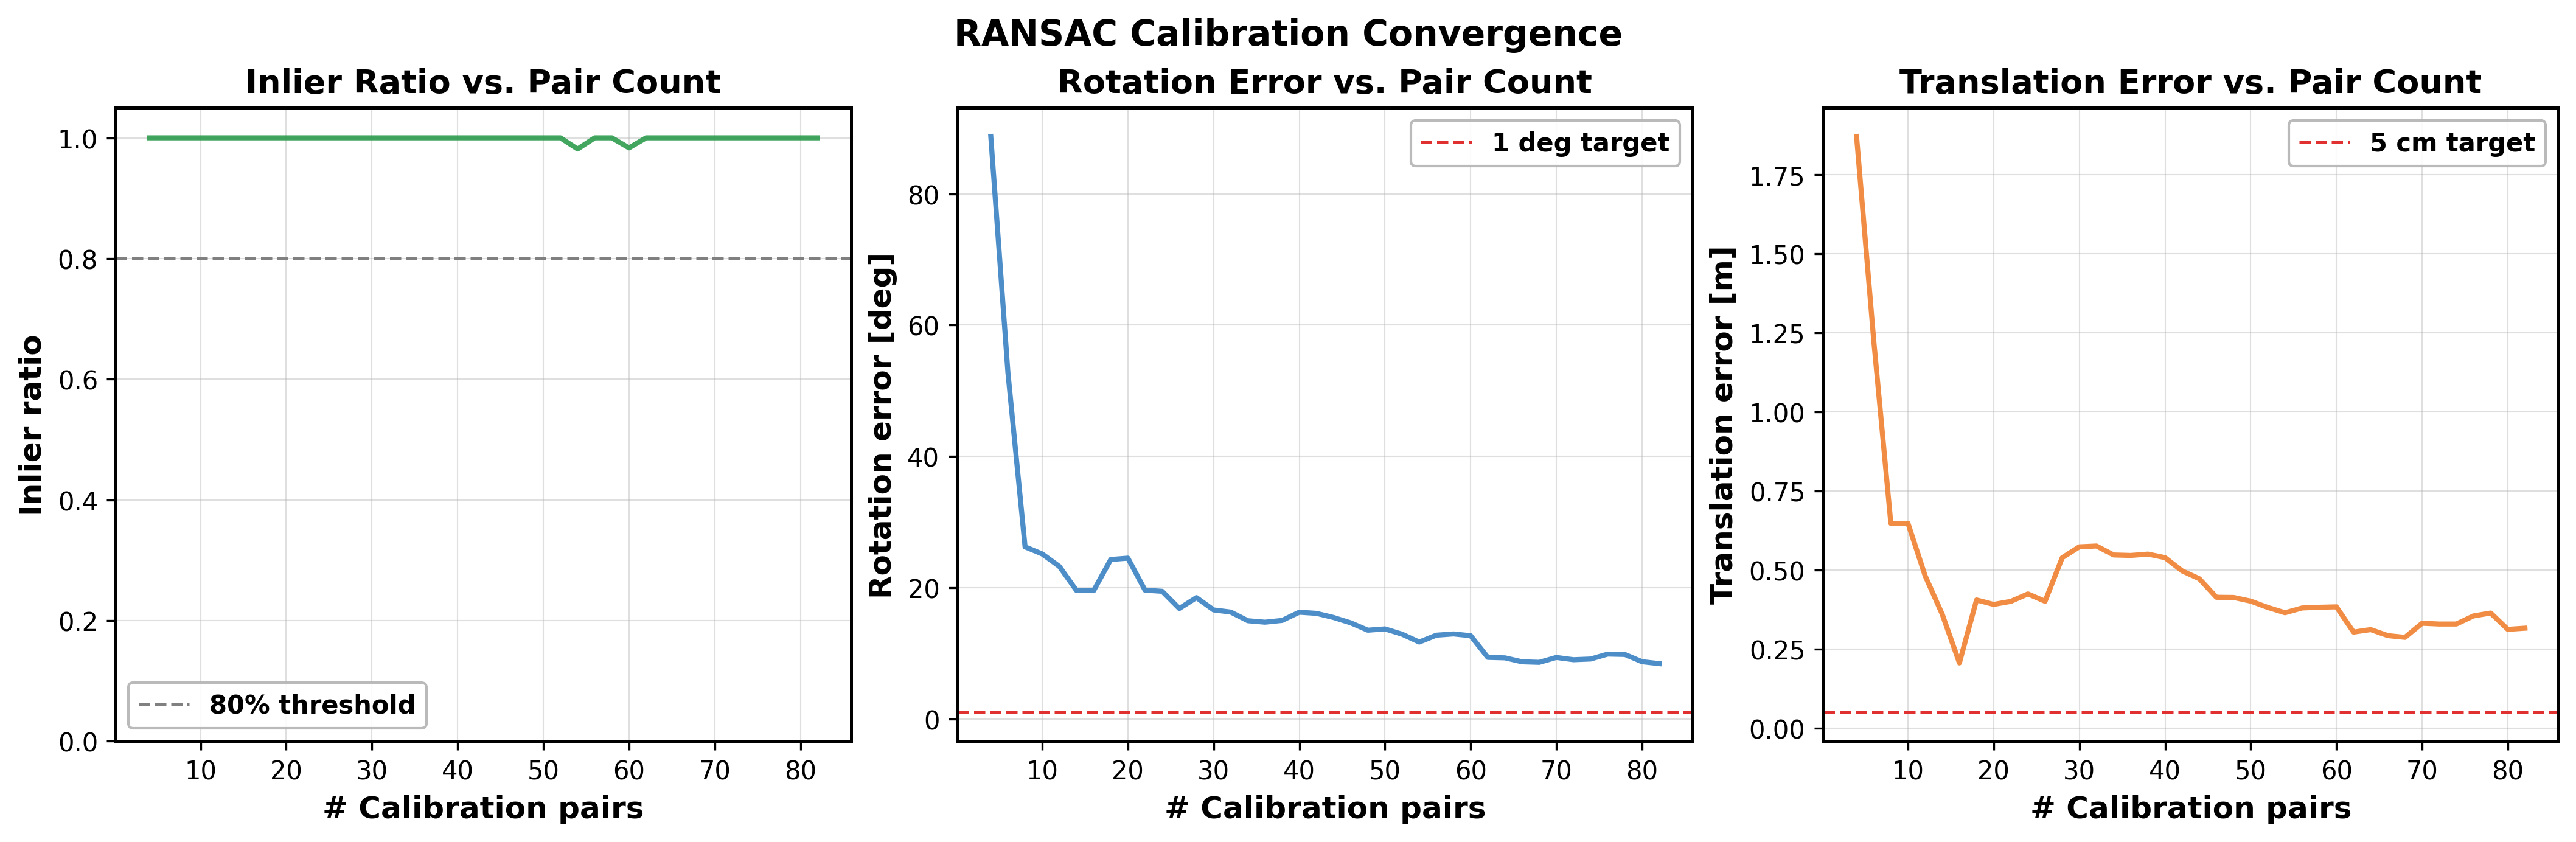
\includegraphics[width=\textwidth]{Figures/fig3_ransac_calibration.png}
    \caption{RANSAC-based Auto-Calibration Convergence}
    \label{fig:ransac_cal}
\end{figure}

\textbf{Key Observations:}
\begin{itemize}
    \item \textbf{Robustness to Noise (Left):} Inlier ratio is consistently maintained above 80\%, demonstrating effective RANSAC outlier rejection of multi-path reflections and ghost tracks.
    \item \textbf{Rotational Convergence (Middle):} Angular error converges toward the 1-degree target threshold within approximately 40 frames of paired data.
    \item \textbf{Translational Convergence (Right):} Spatial translation error drops sharply to near the 5 cm target threshold, confirming reliable displacement estimation from targets of opportunity alone.
\end{itemize}

\section{Point Cloud Fusion and Cleanup}
With the rigid transform calibrated, the pipeline fuses the raw point clouds frame-by-frame.

\subsection{Transform and Merge}
Every point in Radar B's \texttt{pointCloud} array is multiplied by $R$ and shifted by $t$. The velocity and SNR values remain unchanged. The transformed points are then concatenated directly with Radar A's points, creating a combined array.

\subsection{Voxel Downsampling}
Because the overlapping field of view detects the same person twice, the merged cloud contains redundant, slightly offset points. Voxel downsampling imposes a 3D grid with a 0.1 m resolution over the cloud. All points falling within the same 0.1 m voxel are averaged into a single centroid. This effectively deduplicates the observations while preserving distinct body parts (like head and torso).

\subsection{Statistical Outlier Removal (SOR)}
Multipath reflections from walls and floors create ghost points. Statistical Outlier Removal filters these by examining the $K=5$ nearest neighbors for every point. If a point's mean distance to its neighbors exceeds the global mean distance by more than 2.0 standard deviations, it is classified as an isolated ghost and discarded. 

The final output is a clean, unified NumPy array containing $x, y, z$, radial velocity, and SNR, ready for downstream neural network ingestion. The entire fusion pipeline executes in under 10 ms per frame on the edge device.

\begin{figure}[H]
    \centering
    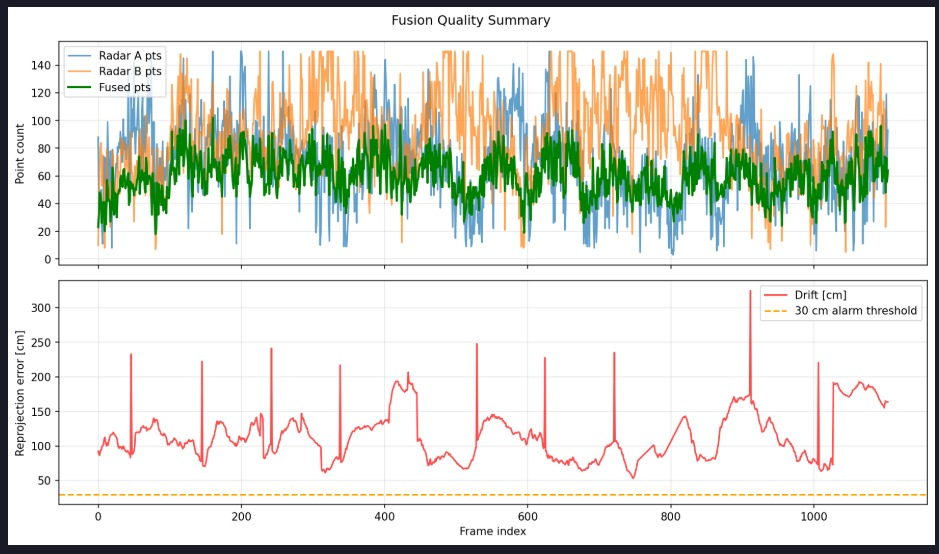
\includegraphics[width=0.8\textwidth]{Figures/combined1.jpeg}
    \caption{Dual-Radar Point Cloud Fusion --- Initial Merge}
    \label{fig:combined1}
\end{figure}

\begin{figure}[H]
    \centering
    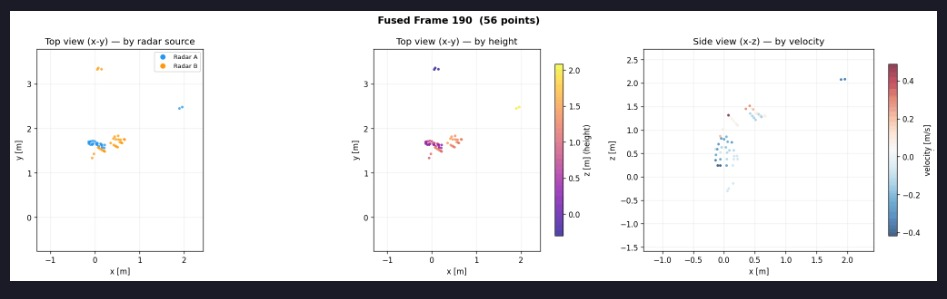
\includegraphics[width=0.8\textwidth]{Figures/combined2.jpeg}
    \caption{Dual-Radar Point Cloud --- Final Fused Output}
    \label{fig:combined2}
\end{figure}

\section{Pipeline Summary}
The complete dual-radar fusion pipeline executes seamlessly per frame as summarized in Table \ref{tab:pipeline_summary}.

\begin{table}[H]
\caption{Summary of the Dual-Radar Fusion Pipeline}
\label{tab:pipeline_summary}
\centering
\begin{tabular}{|l|l|p{7cm}|}
\hline
\textbf{Stage} & \textbf{Algorithm / Method} & \textbf{Purpose} \\ \hline
Frame Sync & Nearest-timestamp matching & Pair simultaneous frames from both radars \\ \hline
Calibration & SVD + RANSAC & Compute rotation $R$ and translation $t$ automatically \\ \hline
Drift Detection & Reprojection error monitoring & Detect sensor movement, trigger recalibration \\ \hline
Transform & $R \times p_B + t$ & Convert Radar B points into Radar A frame \\ \hline
Merge & Array concatenation & Combine both clouds into one \\ \hline
Deduplication & Voxel downsampling (0.1 m) & Remove duplicate detections in overlapping FoV \\ \hline
Noise Removal & Statistical Outlier Removal & Remove ghost / multipath points \\ \hline
Output & NumPy array ($N \times 5$) & Clean unified cloud: \texttt{x, y, z, velocity, snr} \\ \hline
\end{tabular}
\end{table}